% Provenance (never printed): see sources/outline_sources.md (Year 2: ore deposits ---
% magmatic, hydrothermal, sedimentary and supergene deposits; grade and tonnage; exploration).
% Deposit descriptions from the USGS Mineral Deposit Models for Resource Assessment
% (Scientific Investigations Report 2010-5070, chapters A, B, C, E, I, L, N, O, Q), USGS
% Open-File Report 03-077 (orogenic gold) and Grabreck et al. 2022 (kimberlites); the grade and
% tonnage data of the world's porphyry copper deposits from USGS Open-File Report 2008-1155
% (dataset bachelor-2-porphyry-cu). Ledger rows in sources/ledger/book4.md; curves and numbers
% from figdata/bachelor-2/ores.py and the Book 4 second-writer scratch calculator calc/ch29.py.
% Geology and sourced numbers only: no advocacy.
\chapter{अयस्क निक्षेप}\label{ch:b2:ore-deposits}

भूपर्पटी का लगभग \qty{0.006}{\percent} भाग ताँबा है; उसका खनन उस चट्टान से होता है जिसमें लगभग
\qty{0.5}{\percent} ताँबा होता है। इसलिए हर ताँबा खदान ऐसी चट्टान पर बैठी है जो अपने आसपास की भूपर्पटी से
लगभग अस्सी गुना समृद्ध है, और हर \omterm{def:b2:ore-deposits:deposit}{अयस्क निक्षेप} किसी प्राकृतिक सांद्रक का काम है: वह \omterm{def:b2:magma-emplacement:magma}{मैग्मा} जिससे एक
सल्फ़ाइड द्रव अमिश्रणीय होकर अलग हुआ, वह गर्म ब्राइन जिसने धातुएँ घोलीं और उन्हें किसी दरार में छोड़ दिया,
वह नदी जिसने भारी कणों को हल्के कणों से छाँटा, वह वर्षा जिसने किसी अयस्क-पिंड के ऊपरी भाग का निक्षालन किया
और उसके ताँबे को नीचे फिर से निक्षेपित किया। यह अध्याय इन सांद्रकों का अनुसरण करता है, फिर उनके उत्पादों को
मापता है --- कितना अयस्क, किस ग्रेड पर --- और निक्षेपों को खोजने के तरीक़े के साथ समाप्त होता है।
% ledger: perkins:ore-grades

\begin{recall}
\textbf{स्कूल की पुस्तकों से}: \omterm{def:b2:ore-deposits:deposit}{अयस्क निक्षेप} और \omterm{def:b2:ore-deposits:cf}{सांद्रण गुणक}, शिरा, \omterm{def:b2:ore-deposits:placer}{प्लेसर}, भंडार और
संसाधन; जलतापीय परिसंचरण और कटकों पर काले धूम्रक। \textbf{रसायन की पुस्तकों से}: अयस्क;
विलेयता, संकुल आयन और अपचयोपचय। \textbf{पुस्तक 3 (स्नातक वर्ष 1) से}: किसी कण का
अवसादन-वेग और स्टोक्स का नियम; लैटेराइट; वाष्पनिक निक्षेप। \textbf{\cref{ch:b2:elements-in-the-earth}
से}: \omterm{def:b2:elements-in-the-earth:goldschmidt}{ताम्ररागी तत्त्व}, \omterm{def:b2:elements-in-the-earth:partition}{खनिज--गलित विभाजन गुणांक}। \textbf{\cref{ch:b2:magmatic-differentiation}
से}: \omterm{def:b2:magmatic-differentiation:cumulate}{स्तरित अंतर्वेधन} और \omterm{def:b2:magmatic-differentiation:cumulate}{क्यूम्यूलेट}। \textbf{\cref{ch:b2:precambrian-earth} से}: \omterm{def:b2:precambrian-earth:bif}{पट्टित लौह संरचना},
\omterm{def:b2:precambrian-earth:craton}{क्रेटॉन}। \textbf{गणित की पुस्तकों से}: प्रसामान्य और लघुगणकीय-प्रसामान्य बंटन,
और प्रसामान्य
बंटन फलन $\Phi$।
\end{recall}

\section{अयस्क, ग्रेड और सांद्रण}\label{sec:b2:ore-deposits:grade}

\begin{definition}[गैंग]\label{def:b2:ore-deposits:ore}
किसी अयस्क में \emph{गैंग}\index{गैंग} वह सब कुछ है जिसका कोई आर्थिक मूल्य नहीं होता: वे
शैल-निर्माणकारी, जलतापीय और अपक्षय-जनित खनिज जो अयस्क खनिजों के साथ होते हैं और प्रसंस्करण के दौरान
उनसे अलग करके फेंक दिए जाते हैं।
\end{definition}

अधिकांश अयस्क \omterm{def:b2:ore-deposits:ore}{गैंग} ही होता है। \omterm{def:b2:ore-deposits:hydrothermal}{पोर्फ़िरी ताँबा निक्षेप} में, जो विश्व में ताँबे का मुख्य स्रोत है, अयस्क का
\qty{98}{\percent} से अधिक भाग \omterm{def:b2:ore-deposits:ore}{गैंग} होता है, और शेष भाग ताँबे के खनिज हैं।
% ledger: usgs10b:share

\begin{definition}[अयस्क ग्रेड, कट-ऑफ़ ग्रेड, टनभार]\label{def:b2:ore-deposits:grade}
चट्टान के किसी आयतन का \emph{अयस्क ग्रेड}\index{अयस्क ग्रेड} उसमें मूल्यवान तत्त्व या खनिज का
द्रव्यमान-अंश है: आधार धातुओं के लिए प्रतिशत में, सोने, चाँदी और प्लैटिनम-समूह तत्त्वों के लिए ग्राम
प्रति टन में। \emph{कट-ऑफ़ ग्रेड}\index{कट-ऑफ़ ग्रेड} वह न्यूनतम ग्रेड है जिस पर चट्टान के किसी खंड को
अयस्क गिना जाता है; उससे नीचे वह खंड अपशिष्ट है। किसी निक्षेप का
\emph{टनभार}\index{टनभार} कट-ऑफ़ ग्रेड से ऊपर की चट्टान का द्रव्यमान है; अपने माध्य ग्रेड $\bar g$ के
साथ वह अंतर्विष्ट धातु देता है, $M = T\bar g$।
\end{definition}

इसलिए किसी निक्षेप का \omterm{def:b2:ore-deposits:grade}{टनभार} और ग्रेड चट्टान के बारे में दो तथ्य नहीं, बल्कि एक ही प्रश्न के दो उत्तर हैं,
जो किसी दिए गए कट-ऑफ़ पर पूछा जाता है। इंडोनेशिया के पोर्फ़िरी ताँबा--सोना निक्षेप बातू हिजाउ को
\qty{914}{Mt} बताया गया है, \qty{0.53}{\percent} ताँबे के ग्रेड पर, \qty{0.3}{\percent} के कट-ऑफ़ से ऊपर;
और उपलब्ध न्यूनतम कट-ऑफ़ लेने वाले एक विश्व-संकलन में \qty{1640}{Mt}, \qty{0.44}{\percent} पर: कट-ऑफ़
घटाने से \omterm{def:b2:ore-deposits:grade}{टनभार} लगभग दोगुना हो जाता है और माध्य ग्रेड घट जाता है। एक अवसादी जस्ता--सीसा निक्षेप में,
कनाडा के टॉम निक्षेप में, \omterm{def:b2:ore-deposits:grade}{कट-ऑफ़ ग्रेड} को लगभग एक प्रतिशत जस्ता-और-सीसा घटाने से
भंडार पाँच गुना हो जाएँगे।
% ledger: usgs10b:cutoffs, usgs08:tonnage-def, usgs10n:sedex

\begin{definition}[सांद्रण गुणक]\label{def:b2:ore-deposits:cf}
किसी अयस्क में किसी तत्त्व का \emph{सांद्रण गुणक}\index{सांद्रण गुणक} अनुपात $\mathrm{CF} = g/a$ है, अर्थात्
उसके ग्रेड $g$ का किसी संदर्भ आगार में उसकी प्रचुरता $a$ से अनुपात, जिस आगार का उल्लेख साथ में किया जाता है:
समग्र महाद्वीपीय भूपर्पटी, ऊपरी महाद्वीपीय भूपर्पटी, या वह चट्टान जिससे निक्षेप बना।
\end{definition}

गुणक संदर्भ पर निर्भर करता है। भूपर्पटी के लिए \qty{0.006}{\percent} ताँबा और अयस्क के लिए
\qty{0.5}{\percent} लेने पर गुणक 83 आता है; ऊपरी महाद्वीपीय भूपर्पटी, \qty{28}{ppm}, और 2008 का
माध्य पोर्फ़िरी ताँबा ग्रेड, \qty{0.44}{\percent}, लेने पर 157। सोने के गुणक, जो ऊपरी भूपर्पटी में
\qty{1.5}{ng/g} है और कुछ ग्राम प्रति टन पर खनित होता है, हज़ारों में होते हैं; लोहे को, जो भूपर्पटी में
कई प्रतिशत है और लगभग \qty{50}{\percent} पर खनित होता है, केवल लगभग दस के गुणक की
आवश्यकता होती है।
% ledger: perkins:ore-grades, rg03:ucc-trace, usgs10b:share, earle:ore-grades, earle:iron-grade

\begin{definition}[अयस्क निक्षेप]\label{def:b2:ore-deposits:deposit}
\emph{अयस्क निक्षेप}\index{अयस्क निक्षेप} चट्टान का एक ऐसा पिंड है जिसमें प्राकृतिक प्रक्रमों ने किसी तत्त्व या
खनिज को कट-ऑफ़ से ऊपर के ग्रेड तक, इतने बड़े \omterm{def:b2:ore-deposits:grade}{टनभार} पर सांद्रित किया है कि उसे लाभ के साथ निकाला जा
सके। यह एक भूवैज्ञानिक वस्तु भी है, जिसे उसे बनाने वाले प्रक्रम परिभाषित करते हैं, और एक आर्थिक वस्तु भी,
जिसे कीमतें, लागतें और प्रौद्योगिकी परिभाषित करती हैं।
\end{definition}

अपने आर्थिक आधे भाग के कारण किसी निक्षेप का आकार समय के साथ बदलता है। किसी तत्त्व के अभिनिर्धारित
संसाधन वे सांद्रण हैं जिनसे निष्कर्षण अभी संभव है या संभव हो सकता है; उसके भंडार वह भाग हैं जिसे,
उनके निर्धारण के समय, आर्थिक रूप से निकाला जा सकता था। विश्व के ताँबा-भंडार 1970 में \qty{280}{Mt}
थे; तब से लगभग \qty{697}{Mt} का खनन हो चुका है, और 2024 में वे
\qty{980}{Mt} थे।
% ledger: usgs:mcs-reserves

\begin{proposition}[किसी निक्षेप का द्रव्यमान-संतुलन]\label{prop:b2:ore-deposits:mass-balance}
किसी तत्त्व का द्रव्यमान $M$, माध्य ग्रेड $g$ पर, रखने वाले निक्षेप को एक ऐसे स्रोत ने पोषित किया जिसमें
उस तत्त्व की प्रचुरता $a$ थी। यदि सांद्रण प्रक्रम ने स्रोत से तत्त्व का एक अंश $\eta \leq 1$ निकालकर
निक्षेप तक पहुँचाया, तो संसाधित स्रोत-चट्टान का द्रव्यमान था
\begin{equation}
m_{\mathrm{source}} = \frac{M}{\eta\,a} = \frac{\mathrm{CF}}{\eta}\, T ,
\label{eq:b2:ore-deposits:mass-balance}
\end{equation}
जहाँ $T = M/g$ \omterm{def:b2:ore-deposits:grade}{टनभार} है और $\mathrm{CF} = g/a$: अयस्क के प्रति टन पर कम से कम CF टन स्रोत।
\end{proposition}

\begin{proof}
स्रोत ने तत्त्व का $\eta\,a\,m_{\mathrm{source}}$ खोया और निक्षेप ने $M$ पाया; दोनों को बराबर रखने पर
पहला रूप मिलता है, और $M = gT$ से दूसरा। चूँकि $\eta \leq 1$, इसलिए $m_{\mathrm{source}} \geq
\mathrm{CF}\,T$।
\end{proof}

बिंगम कैन्यन, नीचे दिखाया गया पोर्फ़िरी निक्षेप, \qty{3230}{Mt} पर सूचीबद्ध है, \qty{0.882}{\percent}
ताँबे के साथ: \qty{28.5}{Mt} ताँबा। ऊपरी भूपर्पटी के सापेक्ष उसका गुणक 315 है,
और पूर्णतः दक्ष प्रक्रम
को भी औसत ऊपरी भूपर्पटी के \num{1.02e12} टन को रिक्त करना पड़ता, लगभग \qty{377}{km^3}: \qty{7.2}{km}
भुजा वाला एक घन। इसलिए अयस्क बनाने वाले प्रक्रम वे प्रक्रम हैं जो बहुत सारा पदार्थ ---
\omterm{def:b2:magma-emplacement:magma}{मैग्मा}, जल, अवसाद --- एक छोटे आयतन से होकर ले जाते हैं जहाँ तत्त्व फँस जाता है।
% ledger: data:b4-porphyry-cu, rg03:ucc-trace
% values: 28.49 Mt; CF 315; 1.0175e12 t; 377 km3 at 2.7 t/m3; side 7.22 km (calc/ch29.py)

\begin{omfigure}
\centering
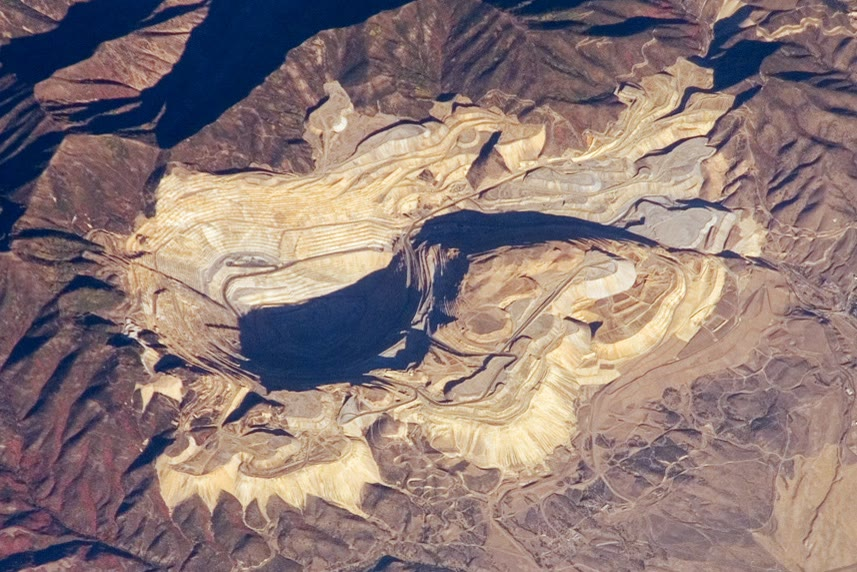
\includegraphics[width=0.5\linewidth]{images/book4/b2-29-bingham-canyon-iss.jpg}
\par\smallskip{\small अंतरराष्ट्रीय अंतरिक्ष स्टेशन से बिंगम कैन्यन की खुली खदान, यूटा
(2007): \qty{4}{km} से अधिक चौड़ी और \qty{1200}{m} गहरी, 16 से \qty{25}{m} ऊँची सीढ़ियों में एक
\omterm{def:b2:ore-deposits:hydrothermal}{पोर्फ़िरी ताँबा निक्षेप} में काटी गई; उसके आसपास की चपटी चोटी वाली पहाड़ियाँ अपशिष्ट चट्टान हैं। फ़ोटो:
NASA, Expedition 15 crew (सार्वजनिक डोमेन)।}
\end{omfigure}
% ledger: photo:b2-29-bingham

\begin{definition}[अयस्क-निक्षेप प्रकार]\label{def:b2:ore-deposits:types}
\emph{अयस्क-निक्षेप प्रकार}\index{अयस्क-निक्षेप प्रकार} निक्षेपों का एक ऐसा वर्ग है जिनमें भूवैज्ञानिक
परिवेश, आतिथेय चट्टान, आकृति, अयस्क का खनिज-संघटन और निर्माण-प्रक्रम साझे होते हैं, ताकि वर्ग का
वर्णन यह पूर्वानुमान दे कि उसके सदस्य कहाँ मिलते हैं। प्रक्रम के अनुसार प्रकार चार कुलों में बँटते हैं:
मैग्मीय (धातु किसी \omterm{def:b2:magma-emplacement:magma}{मैग्मा} द्वारा उसके क्रिस्टलन या अमिश्रण के समय सांद्रित होती है),
जलतापीय (किसी गर्म जलीय तरल द्वारा), अवसादी (अवसाद के परिवहन और निक्षेपण द्वारा,
या सतह पर जल से अवक्षेपण द्वारा), और सुपरजीन (किसी पूर्ववर्ती निक्षेप के
अपक्षय द्वारा)।
\end{definition}

\section{मैग्मीय निक्षेप}\label{sec:b2:ore-deposits:magmatic}

\textbf{स्तरित अंतर्वेधनों में क्रोमाइट।} क्रोमाइट, क्रोमियम का एकमात्र व्यावसायिक स्रोत, स्तरित
अंतर्वेधनों के अल्ट्रामैफ़िक निचले भागों में संहत क्रोमाइटाइट की परतों में जमा होता है, जिनमें
\qty{90}{\percent} से अधिक क्रोमाइट होता है। ये अंतर्वेधन 2 से \qty{180}{km} तक चौड़े और
\qty{15}{km} तक मोटे होते हैं, और परतें एक सेंटीमीटर से कम से लेकर 5--\qty{8}{m} तक होती हैं; मिलकर वे
विश्व के अधिकांश क्रोमियम भंडार रखते हैं, और \cref{ch:b2:magmatic-differentiation} में मिला
बुशवेल्ड संकुल ही आज क्रोमाइट के लिए खनित होने वाला एकमात्र अंतर्वेधन है। उनकी उत्पत्ति --- मैग्माओं के
मिश्रण से, या दाब अथवा ऑक्सीकरण-अवस्था के परिवर्तन से, क्रोमाइट क्षेत्र में धकेली गई एक \omterm{def:b2:magmatic-differentiation:cumulate}{क्यूम्यूलेट} परत ---
अब भी विवादित है।
% ledger: usgs10e:chromite

\textbf{निकेल--ताँबा--PGE सल्फ़ाइड।} प्रावार के बड़े अंश वाले गलन से (\qty{20}{\percent} से \qty{25}{\percent}
या अधिक, भार से 12 प्रतिशत से अधिक MgO के साथ) उत्पन्न कोई मैफ़िक या अल्ट्रामैफ़िक \omterm{def:b2:magma-emplacement:magma}{मैग्मा}
सल्फ़र में असंतृप्त अवस्था में ऊपर उठता है। यदि वह भूपर्पटी से सल्फ़र आत्मसात करे, या पर्याप्त ठंडा हो जाए, तो वह
संतृप्त हो जाता है और एक अमिश्रणीय सल्फ़ाइड द्रव बूँदों के रूप में अलग हो जाता है। ताम्ररागी धातुएँ इन
बूँदों में चली जाती हैं: सल्फ़ाइड द्रव में उनकी सांद्रता और सिलिकेट द्रव में सांद्रता का अनुपात $D$, जो
खनिज और गलित के बीच के विभाजन गुणांक जैसा ही है, ताँबे और निकेल के लिए $10^2$ से $10^3$ और
प्लैटिनम-समूह तत्त्वों के लिए $10^3$ से $10^4$ है। तब कोई बूँद कितनी धातु एकत्र करती है, यह इस पर
निर्भर करता है कि वह कितने \omterm{def:b2:magma-emplacement:magma}{मैग्मा} से मिलती है।
% ledger: usgs10i:r-factor

\begin{proposition}[R-गुणक]\label{prop:b2:ore-deposits:r-factor}
मान लीजिए सल्फ़ाइड द्रव का एक इकाई द्रव्यमान सिलिकेट \omterm{def:b2:magma-emplacement:magma}{मैग्मा} के द्रव्यमान $R$ से, जो \emph{R-गुणक}\index{R-गुणक}
है, एक बंद तंत्र में अलग होता है और उसके साथ साम्य में पहुँचता है; मान लीजिए $C_L$ सल्फ़ाइड के अलग होने से
पहले \omterm{def:b2:magma-emplacement:magma}{मैग्मा} में किसी धातु की सांद्रता है, और $D$ उसका सल्फ़ाइड--सिलिकेट विभाजन
गुणांक। तब सल्फ़ाइड में धातु की सांद्रता है
\begin{equation}
C_S = C_L\,\frac{D\,(R + 1)}{R + D} .
\label{eq:b2:ore-deposits:r-factor}
\end{equation}
$R \gg D$ के लिए $C_S \to D\,C_L$; $R \ll D$ के लिए $C_S \approx (R + 1)\,C_L$।
\end{proposition}

\begin{proof}
द्रव्यमान $R + 1$ के तंत्र में पृथक्करण से पहले धातु की मात्रा $(R + 1)C_L$ थी। उसके बाद सिलिकेट में
$R\,C_{\mathrm{sil}}$ और सल्फ़ाइड में $C_S$ है, साम्य पर $C_S = D\,C_{\mathrm{sil}}$ के साथ।
संरक्षण से $(R + 1)C_L = R\,C_S/D + C_S = C_S\,(R + D)/D$ मिलता है, अतः
\eqref{eq:b2:ore-deposits:r-factor}। यदि $R \gg D$, तो $(R + 1)/(R + D) \to 1$; यदि $R \ll D$, तो
$D/(R + D) \to 1$।
\end{proof}

दोनों सीमाएँ समझाती हैं कि सल्फ़ाइड अयस्क दो प्रकार के क्यों होते हैं। जब $R \ll D$, तो सल्फ़ाइड जिस \omterm{def:b2:magma-emplacement:magma}{मैग्मा} से
मिलता है उसकी लगभग सारी धातु ले लेता है और $C_S$, $R$ के साथ बढ़ता है; जब $R \gg D$, तो वह $D\,C_L$ पर
संतृप्त होता है और अधिक \omterm{def:b2:magma-emplacement:magma}{मैग्मा} कुछ नहीं जोड़ता। निकेल और ताँबा, जिनका $D$ कुछ सौ है, कुछ सौ से कुछ हज़ार के
$R$ पर अपनी अधिकतम सीमा तक पहुँच जाते हैं, जो अधिकांश निकेल--ताँबा अयस्कों का परास है; प्लैटिनम और पैलेडियम,
जिनका $D$ लगभग $10^4$ है, $R$ के \num{10000} से \num{100000} तक पहुँचने तक धातु पाते रहते हैं। इसलिए
प्लैटिनम-समूह तत्त्वों से समृद्ध अयस्क, जैसे बुशवेल्ड की मेरेंस्की रीफ़ और नोरिल्स्क के कुछ अयस्क, सल्फ़ाइड के
एक छोटे द्रव्यमान को दर्ज करते हैं जिसे \omterm{def:b2:magma-emplacement:magma}{मैग्मा} के एक बहुत बड़े द्रव्यमान ने धोया
(अभ्यास~\ref{exo:b2:ore-deposits:5} और~\ref{exo:b2:ore-deposits:11})।
% ledger: usgs10i:r-factor

\textbf{किंबरलाइट और हीरे।} अधिकांश हीरे, और लगभग सभी खनित हीरे, मोटे महाद्वीपीय स्थलमंडल के आधार पर,
\omterm{def:b2:precambrian-earth:craton}{क्रेटॉनों} की जड़ों में बने; किंबरलाइट \omterm{def:b2:magma-emplacement:magma}{मैग्मा}, जो 120 से \qty{150}{km} से अधिक गहराई से आते हैं और
\qty{20}{m.s^{-1}} तक की गति से ऊपर उठते हैं, उन्हें इतनी तेज़ी से सतह तक लाते हैं कि वे बचे रहें।
किंबरलाइट वरीयता से मोटे, पुराने स्थलमंडल से होकर उद्गारित होते हैं, और हीरों की खोज
वहीं की जाती है।
% ledger: grabreck22:kimberlite

\textbf{पेग्मेटाइट।} लिथियम--सीज़ियम--टैंटलम पेग्मेटाइट इन दुर्लभ तत्त्वों से समृद्ध ग्रेनाइटी \omterm{def:b2:magma-emplacement:bodies}{डाइक} हैं, जो
टक्कर वाली \omterm{def:b2:alpine-orogen:orogen}{पर्वतजनक पट्टियों} में बनते हैं; वे लगभग 350 से \qty{550}{\celsius} पर, जो किसी ग्रेनाइटी गलित के
लिए उल्लेखनीय रूप से कम है, दिनों से वर्षों में क्रिस्टलित होते हैं, और विशाल क्रिस्टल उगाते हैं --- स्पोड्यूमीन
का एक क्रिस्टल \qty{14}{m} लंबा था। उनके लिथियम खनिज, स्पोड्यूमीन, पेटालाइट और लेपिडोलाइट, विश्व के
लगभग एक-चौथाई लिथियम की आपूर्ति करते हैं।
% ledger: usgs10o:lct

\section{जलतापीय निक्षेप}\label{sec:b2:ore-deposits:hydrothermal}

\begin{definition}[जलतापीय तरल और जलतापीय निक्षेप प्रकार]\label{def:b2:ore-deposits:hydrothermal}
\emph{जलतापीय तरल}\index{जलतापीय तरल} एक गर्म जलीय तरल है --- किसी \omterm{def:b2:magma-emplacement:magma}{मैग्मा} द्वारा या कायांतरी अभिक्रियाओं द्वारा
मुक्त, या गर्म किया गया समुद्री जल, उल्कीय जल या द्रोणी-ब्राइन --- जो चट्टान से होकर बहते हुए तत्त्वों को
घोलता, परिवहित करता और निक्षेपित करता है। मुख्य जलतापीय \omterm{def:b2:ore-deposits:types}{अयस्क-निक्षेप प्रकार}
ये हैं:
\begin{itemize}
  \item \emph{पोर्फ़िरी ताँबा निक्षेप}\index{पोर्फ़िरी ताँबा निक्षेप}: एक छोटे पोर्फ़िरी स्टॉक के भीतर और
        आसपास शिरिकाओं और प्रसारित ताँबा सल्फ़ाइडों का एक बड़ा, निम्न-ग्रेड पिंड, जो किसी क्षेपण क्षेत्र के
        ऊपर सतह से कुछ किलोमीटर के भीतर मैग्मीय तरलों द्वारा बना;
  \item \emph{एपिथर्मल निक्षेप}\index{एपिथर्मल निक्षेप}: सोना--चाँदी की शिराएँ और प्रसारित खनिजन,
        जो ज्वालामुखी चापों में, सतह से लगभग \qty{1.5}{km} के भीतर, लगभग 100 से
        \qty{300}{\celsius} पर बनते हैं;
  \item \emph{ज्वालामुखीजनित संहत सल्फ़ाइड निक्षेप}\index{ज्वालामुखीजनित संहत सल्फ़ाइड निक्षेप}
        (VMS): संहत सल्फ़ाइडों का एक लेंस, जो किसी समुद्री ज्वालामुखीय परिवेश में किसी जलतापीय
        निकास-छिद्र पर, समुद्र-तल पर या उसके ठीक नीचे बनता है;
  \item \emph{अवसादी उच्छ्वासी निक्षेप}\index{अवसादी उच्छ्वासी निक्षेप} (सेडेक्स):
        किसी \omterm{def:b2:basins-compared:types}{दरार-द्रोणी} की समुद्री शेलों में पटलित जस्ता--सीसा सल्फ़ाइड, जो भ्रंशों के अनुदिश ऊपर उठते
        द्रोणी-ब्राइनों से समुद्र-तल पर या उसके ठीक नीचे अवक्षेपित होते हैं;
  \item \emph{मिसिसिपी घाटी-प्रकार निक्षेप}\index{मिसिसिपी घाटी-प्रकार निक्षेप} (MVT):
        प्लेटफ़ॉर्म कार्बोनेटों का प्रतिस्थापन करते जस्ता--सीसा सल्फ़ाइड, जो पश्चजात हैं और आग्नेय
        सक्रियता से असंबद्ध हैं, और द्रोणी-ब्राइनों द्वारा निक्षेपित होते हैं;
  \item \emph{पर्वतजनक स्वर्ण निक्षेप}\index{पर्वतजनक स्वर्ण निक्षेप}: कायांतरी पट्टियों में, बड़े भ्रंशों के
        अनुदिश, सोना-युक्त क्वार्ट्ज़ शिराएँ, जो कायांतरी उत्पत्ति के कम-लवणता वाले, CO$_2$-समृद्ध तरलों
        द्वारा निक्षेपित होती हैं।
\end{itemize}
\end{definition}
% ledger: usgs10b:form, usgs10q:epithermal, usgs10c:vms, usgs10n:sedex, usgs10a:mvt, drew03:orogenic

\textbf{परिवहन और निक्षेपण।} अधिकांश धातुएँ जलतापीय तरलों में संकुलों के रूप में ले जाई जाती हैं: जस्ता,
सीसा और ताँबा क्लोराइड संकुलों के रूप में, जिससे लवणता उनकी विलेयता को नियंत्रित करती है, और सोना,
अपचयित तरलों में, AuHS(H$_2$S)$_3$ जैसे सल्फ़र संकुलों के रूप में। कोई तरल अपना भार तब छोड़ता है जब
विलेयता घटती है: जब वह ठंडा होता है; जब दाब घटने पर वह उबलता है, H$_2$S और CO$_2$ खोता है और उसका pH
बदलता है; जब वह भिन्न संघटन वाले किसी तरल से मिलता है --- H$_2$S से समृद्ध जल से मिलने वाला ब्राइन
स्फैलेराइट और गैलेना को लगभग तुरंत अवक्षेपित कर देता है; और जब वह भित्ति-चट्टान से अभिक्रिया करता है,
जिससे उसका pH या ऑक्सीकरण-अवस्था बदलती है। हर निक्षेप प्रकार तरल, मार्ग और फंदे का
एक संयोजन है।
% ledger: usgs10n:sedex, drew03:orogenic

\textbf{पोर्फ़िरी ताँबा।} पोर्फ़िरी निक्षेप विश्व के लगभग \qty{60}{\percent} ताँबे की आपूर्ति करते हैं और
उसके लगभग \qty{65}{\percent} संसाधन रखते हैं। उनके केंद्र में छोटे बेलनाकार स्टॉक या \omterm{def:b2:magma-emplacement:bodies}{डाइकों} के झुंड
होते हैं, जो बड़े \omterm{def:b2:magma-emplacement:bodies}{प्लूटॉनों} के शीर्ष हैं और क्षेपण क्षेत्रों के ऊपर के चापों में 5--\qty{10}{km} से कम
गहराई पर स्थापित हुए, जो \cref{ch:b2:magmatic-series} का परिवेश है। एक निक्षेप 0.1 से
\qty{1}{km} तक चौड़ा होता है, लगभग उतनी ही ऊँचाई के साथ; परिवर्तित चट्टान उसके चारों ओर \qty{10}{km}
या अधिक तक फैल सकती है। जैसे-जैसे \omterm{def:b2:magma-emplacement:magma}{मैग्मा} क्रिस्टलित होता है, भार से 3 से 5 प्रतिशत लवण वाला एक तरल
उससे अलग होता है; ऊपर उठते और विसंपीडित होते हुए वह एक ब्राइन और एक वाष्प में बँट जाता है, दोनों धातुएँ
ले जाते हैं, और उसका अतिदाब चट्टान को तोड़ देता है। क्वार्ट्ज़ शिराएँ लगभग 700 से \qty{500}{\celsius} पर
अवक्षेपित होती हैं, और चट्टान के साथ तरल की अभिक्रिया परिवर्तन को क्षेत्रों में बाँटती है, जैसा नीचे के
खंड-चित्र में है। चूँकि वे सक्रिय किनारों पर उथली गहराई में बनते हैं, जहाँ अपरदन तेज़ है, इसलिए ज्ञात
पोर्फ़िरी निक्षेपों में से \qty{90}{\percent} से अधिक सीनोज़ोइक या मेसोज़ोइक हैं।
% ledger: usgs10b:share, usgs10b:form, usgs10b:fluids, usgs10b:alteration

\begin{omfigure}
\centering
\begin{tikzpicture}[x=1.15cm, y=1.15cm, font=\small]
\begin{scope}
\clip (-2.9,-3.6) rectangle (2.9,0);
% propylitic halo
\fill[omLithBasalt!45] (0,-1.25) ellipse (2.45 and 1.55);
% sodic-calcic deep flanks
\fill[omExo!25] (-1.75,-2.55) ellipse (0.45 and 0.38);
\fill[omExo!25] (1.75,-2.55) ellipse (0.45 and 0.38);
% sericitic shell
\fill[yellow!35] (0,-1.05) ellipse (1.15 and 1.15);
% potassic core
\fill[omProp!40] (0,-1.45) ellipse (0.68 and 0.85);
% ore shell
\draw[omThm, line width=1.1pt, densely dashed] (0,-1.3) ellipse (0.92 and 0.98);
% advanced argillic lithocap
\fill[omDef!30] (-1.05,0) .. controls (-0.6,-0.5) and (0.6,-0.5) .. (1.05,0) -- cycle;
\draw[omDef!70] (-1.05,0) .. controls (-0.6,-0.5) and (0.6,-0.5) .. (1.05,0);
\end{scope}
% pluton and stock
\fill[omLithGranite] (-2.6,-3.6) .. controls (-2.2,-2.9) and (-0.9,-2.6) .. (-0.3,-2.6)
  -- (-0.3,-1.25) arc[start angle=180, end angle=0, radius=0.3] -- (0.3,-2.6)
  .. controls (0.9,-2.6) and (2.2,-2.9) .. (2.6,-3.6) -- cycle;
\draw[black!60] (-2.6,-3.6) .. controls (-2.2,-2.9) and (-0.9,-2.6) .. (-0.3,-2.6)
  -- (-0.3,-1.25) arc[start angle=180, end angle=0, radius=0.3] -- (0.3,-2.6)
  .. controls (0.9,-2.6) and (2.2,-2.9) .. (2.6,-3.6);
% epithermal veins
\foreach \x in {1.45,1.65,1.85} \draw[omDef, line width=1pt] (\x,-0.02) -- (\x+0.12,-0.7);
% palaeosurface
\draw[black, line width=0.8pt] (-2.9,0) -- (2.9,0);
\node[anchor=south west, font=\scriptsize] at (-2.9,0) {पुरासतह};
% labels
\draw[black!50] (0.6,-0.15) -- (1.2,0.25) -- (3.0,0.25) node[anchor=west, text=black] {उन्नत आर्जिलिक};
\draw[black!50] (1.95,-0.3) -- (3.0,-0.3) node[anchor=west, text=black] {एपिथर्मल शिराएँ};
\draw[black!50] (1.05,-0.8) -- (3.0,-0.8) node[anchor=west, text=black] {सेरिसिटिक};
\draw[black!50] (0.85,-1.25) -- (3.0,-1.25) node[anchor=west, text=omThm] {ताँबा अयस्क कवच};
\draw[black!50] (0.45,-1.7) -- (3.0,-1.7) node[anchor=west, text=black] {पोटैसिक};
\draw[black!50] (1.05,-2.15) -- (3.0,-2.15) node[anchor=west, text=black] {प्रोपिलिटिक};
\draw[black!50] (2.1,-2.6) -- (3.0,-2.6) node[anchor=west, text=black] {सोडिक--कैल्सिक};
\draw[black!50] (1.5,-3.15) -- (3.0,-3.15) node[anchor=west, text=black] {प्लूटॉन और पोर्फ़िरी स्टॉक};
\end{tikzpicture}
\par\smallskip{\small खंड में एक पोर्फ़िरी ताँबा तंत्र (एक रेखाचित्र, पैमाने पर नहीं): पोटैसिक
क्षेत्र केंद्र में, गहरा और गर्म; सेरिसिटिक क्षेत्र ऊपर और बाहर की ओर, जहाँ पायराइट
प्रचुर है; उनके बीच ताँबा अयस्क कवच; चारों ओर उथली से मध्यम गहराइयों पर प्रोपिलिटिक घेरा;
गहरे पार्श्वों पर सोडिक--कैल्सिक परिवर्तन; एक उन्नत आर्जिलिक टोपी और, कुछ
तंत्रों में, सतह के निकट एपिथर्मल शिराएँ।}
\end{omfigure}
% ledger: usgs10b:alteration

\textbf{एपिथर्मल सोना।} कुछ पोर्फ़िरी तंत्रों के ऊपर, और सामान्यतः ज्वालामुखी चापों में, उसी प्रकार के
तरल भूपर्पटी के ऊपरी \qty{1.5}{km} तक लगभग 100 से \qty{300}{\celsius} पर पहुँचते हैं, जहाँ वे उबलते हैं
और भूजल से मिलते हैं; वे क्वार्ट्ज़ शिराओं में सोना और चाँदी निक्षेपित करते हैं, ऐसे परिवर्तन के साथ जो
लगभग उदासीन तरलों (एड्यूलेरिया, इलाइट) या बहुत अम्लीय तरलों (केओलिनाइट, डिकाइट, पायरोफ़िलाइट) को
दर्ज करता है।
% ledger: usgs10q:epithermal, usgs10q:alteration

\textbf{समुद्र-तल पर संहत सल्फ़ाइड।} किसी कटक या चाप की गर्म भूपर्पटी में नीचे खिंचा समुद्री जल लगभग
\qty{350}{\celsius} पर काले धूम्रकों के रूप में निकास-छिद्रों से लौटता है; ये पहली बार 1979 में पूर्वी प्रशांत
उभार पर देखे गए। जहाँ निकास-क्षेत्र टिका रहता है, वहाँ उसके सल्फ़ाइड एक टीला बनाते हैं; अयस्क में
\qty{40}{\percent} से अधिक सल्फ़ाइड होते हैं, जो शिराओं के एक स्टॉकवर्क के ऊपर स्थित है जो पोषक मार्ग को
चिह्नित करता है। धातुएँ तापमान के अनुसार क्षेत्रित हैं: गर्म आधार पर लोहा और ताँबा, अधिक ठंडे शीर्ष और
किनारों पर जस्ता, लोहा, सीसा और बेरियम, जैसा कि अगले खंड में बनाए गए टीले में है। \omterm{def:b2:ore-deposits:hydrothermal}{ज्वालामुखीजनित संहत
सल्फ़ाइड निक्षेप} एक टन से कम के पिंडकों से लेकर स्पेन के रियो टिंटो के \qty{1.5}{Gt} तक होते हैं, और आयु
में \qty{3.55}{\Ga} से लेकर आज बन रहे निक्षेपों तक।
% ledger: usgs10c:vms

\textbf{द्रोणी-ब्राइन: सेडेक्स और MVT।} 10 से \qty{30}{\percent} घुले लवणों वाले द्रोणी-ब्राइन, दबने से
100--\qty{200}{\celsius} तक गर्म होकर, जस्ता और सीसा क्लोराइड संकुलों के रूप में ले जाते हैं और दोनों
अवसाद-आतिथेय प्रकार बनाते हैं। सेडेक्स निक्षेप वहाँ बनते हैं जहाँ ब्राइन किसी दरार-भ्रंश के अनुदिश किसी
सीमित, अपचयित द्रोणी में निकलता है और हाइड्रोजन सल्फ़ाइड से मिलता है, जिससे पटलित सल्फ़ाइड पंक बनते हैं;
वे विश्व के जस्ता और सीसा भंडारों का आधे से अधिक भाग रखते हैं। MVT निक्षेप वहाँ बनते हैं जहाँ किसी द्रोणी
से बाहर धकेला गया ब्राइन उसके किनारे पर किसी कार्बोनेट प्लेटफ़ॉर्म तक पहुँचता है और 75 से लगभग
\qty{200}{\celsius} पर उसका प्रतिस्थापन करता है; वे अवसाद-आतिथेय निक्षेपों के सीसे और जस्ते का
\qty{38}{\percent} रखते हैं, जिनमें जस्ता सीसे से लगभग दस गुना अधिक है।
% ledger: usgs10n:sedex, usgs10a:mvt

\textbf{पर्वतजनक सोना।} कायांतरी पट्टियों में वाष्पशील-निष्कासन अभिक्रियाएँ CO$_2$ से समृद्ध एक लगभग
उदासीन, कम-लवणता वाला तरल मुक्त करती हैं; बड़े भ्रंशों के अनुदिश प्रवाहित होकर वह लगभग \qty{350}{\celsius}
और 4 से \qty{12}{km} गहराई पर सोना-युक्त क्वार्ट्ज़ शिराएँ निक्षेपित करता है। ये शिराएँ बड़ी ऊँचाइयों तक
अविच्छिन्न हैं: भारत में कोलार में \qty{3.2}{km}।
% ledger: drew03:orogenic

\section{अवसादी और सुपरजीन निक्षेप}\label{sec:b2:ore-deposits:sedimentary}

\begin{definition}[प्लेसर]\label{def:b2:ore-deposits:placer}
\emph{प्लेसर}\index{प्लेसर} सघन, टिकाऊ खनिजों का एक अवसादी निक्षेप है जिन्हें बहता जल या पवन
सांद्रित करता है, क्योंकि समान आकार पर वे अपने आसपास के क्वार्ट्ज़ कणों की तुलना में तेज़ी से बैठते हैं और
कम आसानी से प्रवाह में उठाए जाते हैं।
\end{definition}

लगभग 2.85 से अधिक घनत्व वाले खनिज भारी कहलाते हैं, जबकि क्वार्ट्ज़ का 2.65 है: इल्मेनाइट और ज़िरकॉन
लगभग 4.7, मैग्नेटाइट 5.2, सोना 15 से 19.3। स्टोक्स के नियम से किसी कण का अवसादन-वेग उसके अतिरिक्त
घनत्व $\rho_s - \rho_w$ के साथ बढ़ता है, जो सोने के लिए क्वार्ट्ज़ से ग्यारह गुना बड़ा है, इसलिए किसी दिए
गए आकार का सोना अपने से तीन गुना बड़े क्वार्ट्ज़ के साथ रहता है (अभ्यास~\ref{exo:b2:ore-deposits:3}); सोना
प्रायः आधार-चट्टान पर नदी की बजरी में रहता है, जबकि इल्मेनाइट, रूटाइल और ज़िरकॉन समुद्र-तटों और टीलों तक
पहुँचते हैं। भारी-खनिज रेतों में ग्रेड भारी खनिजों का भार-प्रतिशत होता है।
% ledger: usgs10l:heavy, usgs:gold-placer

रासायनिक अवसाद भी अयस्क हैं। \cref{ch:b2:precambrian-earth} की पट्टित लौह संरचनाएँ, जो महासागरों के
घुले लोहे के ऑक्सीकृत होने पर अवक्षेपित हुईं, लोहे का एक सामान्य अयस्क हैं; वाष्पनिक निक्षेप हैलाइट और
पोटैशियम लवण देते हैं; लैटेराइट, जो गहरे उष्णकटिबंधीय अपक्षय का अवशेष हैं, ऐलुमिनियम को बॉक्साइट के रूप
में सांद्रित करते हैं। अपक्षय पहले के निक्षेपों को समृद्ध भी करता है।
% ledger: earle:bif, usgs:bauxite

\begin{definition}[सुपरजीन संवर्धन, गॉसन]\label{def:b2:ore-deposits:supergene}
\emph{सुपरजीन संवर्धन}\index{सुपरजीन संवर्धन} नीचे उतरते भूजल द्वारा किसी धातु का सांद्रण है: जलस्तर के
ऊपर ऑक्सीजनयुक्त, अम्लीय जल किसी अयस्क-पिंड के सल्फ़ाइडों से धातु को घोलता है, और उसके नीचे, अपचायी
परिस्थितियों में, उसे फिर से निक्षेपित करता है, अधिकतर प्राथमिक सल्फ़ाइडों का प्रतिस्थापन करके।
\emph{गॉसन}\index{गॉसन} वह सरंध्र, लौह-ऑक्साइड-समृद्ध चट्टान है जो किसी अपक्षयित सल्फ़ाइड पिंड के ऊपर
सतह पर बची रहती है, जिसके सल्फ़ाइडों का स्थान गोएथाइट, हेमेटाइट और
जैरोसाइट ने ले लिया है।
\end{definition}

पोर्फ़िरी निक्षेपों में जलस्तर के ऊपर का निक्षालित आवरण कई सौ मीटर तक मोटा होता है; उसके नीचे, कैल्कोसाइट
के संवर्धित सल्फ़ाइड क्षेत्र, दसियों से कई सौ मीटर मोटे, \qty{1.5}{Gt} से अधिक तक पहुँचते हैं, 0.4 से
\qty{1.7}{\percent} ताँबे पर, जो नीचे के प्राथमिक, हाइपोजीन अयस्क से सदा अधिक समृद्ध होते हैं। \omterm{def:b2:ore-deposits:supergene}{गॉसन} और
निक्षालित आवरण के लौह ऑक्साइड उन सल्फ़ाइडों की बनावट बनाए रखते हैं जिनका उन्होंने प्रतिस्थापन किया, और
नीचे की खोज का मार्गदर्शन करते हैं; \omterm{def:b2:ore-deposits:supergene}{गॉसनों} और उनके लौह-धब्बों ने आरंभिक खनिकों को कई संहत सल्फ़ाइड
निक्षेपों का पता दिया।
% ledger: usgs10b:supergene, usgs10c:vms

\begin{omfigure}
\centering
\begin{minipage}[b]{0.46\linewidth}\centering
\begin{tikzpicture}[x=1cm, y=1cm, font=\scriptsize]
\fill[omHist!55] (0,4.0) rectangle (1.8,5.2);
\fill[omMeth!30] (0,3.0) rectangle (1.8,4.0);
\fill[black!55] (0,1.8) rectangle (1.8,3.0);
\fill[black!18] (0,0) rectangle (1.8,1.8);
\draw (0,0) rectangle (1.8,5.2);
\draw[omDef, line width=1pt, densely dashed] (-0.25,3.0) -- (2.05,3.0);
\foreach \x in {0.45,0.9,1.35} \draw[omDef, -{Stealth[length=4pt]}] (\x,5.0) -- (\x,3.2);
\node[anchor=west, align=left] at (2.0,4.6) {गॉसन और निक्षालित\\आवरण (Fe ऑक्साइड)};
\node[anchor=west, align=left] at (2.0,3.5) {ऑक्साइड क्षेत्र\\(मैलेकाइट)};
\node[anchor=east, text=omDef, align=right] at (-0.25,3.0) {जलस्तर};
\node[anchor=west, align=left] at (2.0,2.4) {संवर्धन परत\\(कैल्कोसाइट)};
\node[anchor=west, align=left] at (2.0,0.9) {प्राथमिक अयस्क\\(कैल्कोपायराइट\\+ पायराइट)};
\node[anchor=south, font=\scriptsize, text=omDef] at (0.9,5.25) {अम्लीय जल, Cu$^{2+}$};
\end{tikzpicture}
\end{minipage}\hfill
\begin{minipage}[b]{0.52\linewidth}\centering
\begin{tikzpicture}[x=1cm, y=1cm, font=\scriptsize]
\fill[omSea] (-2.6,1.4) rectangle (2.6,3.2);
\fill[omLithBasalt!60] (-2.6,-1.6) rectangle (2.6,1.4);
% stockwork cone
\fill[omProp!25] (-0.5,-1.6) -- (0.5,-1.6) -- (1.1,0.9) -- (-1.1,0.9) -- cycle;
\foreach \x/\y in {-0.3/-1.2,0.1/-1.0,-0.6/-0.4,0.4/-0.3,-0.1/0.1,0.6/0.4,-0.7/0.5}
  \draw[omProp!80!black] (\x,\y) -- ++(0.35,0.25);
% mound: upper rim and core
\fill[yellow!45] (-1.8,1.4) .. controls (-1.2,2.35) and (1.2,2.35) .. (1.8,1.4) -- cycle;
\fill[omThm!45] (-1.1,1.4) .. controls (-0.7,2.0) and (0.7,2.0) .. (1.1,1.4) -- cycle;
\draw (-1.8,1.4) .. controls (-1.2,2.35) and (1.2,2.35) .. (1.8,1.4);
% chimney and plume
\fill[black!70] (-0.08,2.1) rectangle (0.08,2.55);
\fill[black!45] (0,2.6) circle (0.12) (0.1,2.8) circle (0.16) (0.25,3.0) circle (0.2);
\draw[omDef, -{Stealth[length=4pt]}] (-2.3,2.9) -- (-2.3,0.2) -- (-1.2,-0.9);
\draw[omThm, -{Stealth[length=4pt]}] (0,-1.5) -- (0,1.2);
\node[anchor=west, text=omDef] at (-2.55,3.05) {समुद्री जल};
\node[anchor=west] at (0.45,2.85) {काला धूम्रक, \qty{350}{\celsius}};
\draw[black!50] (1.45,1.75) -- (2.0,2.15) node[anchor=west, text=black] {Zn, Fe, Pb, Ba};
\draw[black!50] (0.6,1.6) -- (2.0,1.15) node[anchor=west, text=black] {Fe, Cu};
\node[anchor=west, align=left] at (0.95,-0.4) {स्टॉकवर्क\\(पोषक)};
\node[anchor=north, text=omThm] at (0,-1.6) {गर्म तरल};
\end{tikzpicture}
\end{minipage}
\par\smallskip{\small बाएँ: किसी ताँबा सल्फ़ाइड पिंड के ऊपर एक सुपरजीन परिच्छेदिका (एक रेखाचित्र, पैमाने पर
नहीं): अम्लीय जल जलस्तर के ऊपर ताँबे का निक्षालन करता है और उसे नीचे कैल्कोसाइट के रूप में फिर से
निक्षेपित करता है, सतह पर एक \omterm{def:b2:ore-deposits:supergene}{गॉसन} छोड़ते हुए। दाएँ: खंड में एक ज्वालामुखीजनित संहत सल्फ़ाइड टीला (एक
रेखाचित्र): भूपर्पटी में गर्म हुआ समुद्री जल एक स्टॉकवर्क से होकर ऊपर उठता है और काले धूम्रक के रूप में
निकलता है; टीला गर्म आधार पर लोहे और ताँबे से लेकर शीर्ष और किनारों पर जस्ता, लोहा, सीसा और बेरियम तक
क्षेत्रित है।}
\end{omfigure}
% ledger: usgs10b:supergene, usgs10c:vms

\begin{omfigure}
\centering
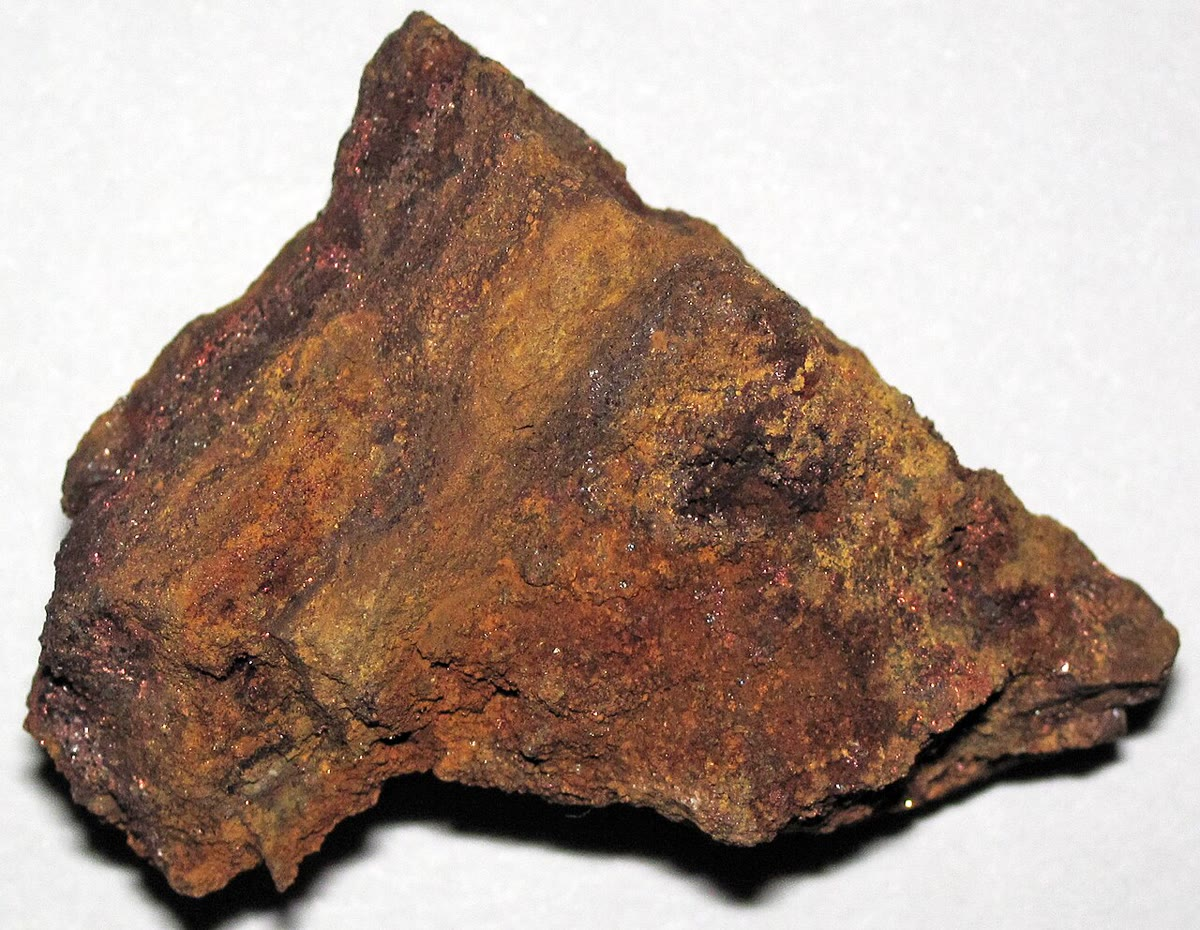
\includegraphics[width=0.4\linewidth]{images/book4/b2-29-flambeau-gossan.jpg}
\par\smallskip{\small विस्कॉन्सिन के फ़्लैम्बो संहत सल्फ़ाइड निक्षेप का \omterm{def:b2:ore-deposits:supergene}{गॉसन}: लौह हाइड्रॉक्सी-ऑक्साइडों की
एक सरंध्र चट्टान, जो एक पैलियोप्रोटेरोज़ोइक ज्वालामुखी चाप में पायराइट, कैल्कोपायराइट, कैल्कोसाइट और
बोर्नाइट के अपक्षय से बची; छोटे नारंगी धब्बे प्राकृत ताँबा हैं। फ़ोटो: James St.~John,
CC BY 2.0।}
\end{omfigure}
% ledger: photo:b2-29-gossan

\section{ग्रेड और टनभार}\label{sec:b2:ore-deposits:grade-tonnage}

एक विश्व-संकलन 422 \omterm{def:b2:ore-deposits:hydrothermal}{पोर्फ़िरी ताँबा निक्षेपों} को उनके \omterm{def:b2:ore-deposits:grade}{टनभार} के साथ, उपलब्ध न्यूनतम कट-ऑफ़ पर, और उनके
माध्य ताँबा ग्रेड के साथ सूचीबद्ध करता है। उनमें से दसवाँ भाग \qty{1500}{Mt} से अधिक है और दसवें भाग में
\qty{33}{Mt} से कम है, माध्यिका \qty{240}{Mt} के साथ; उन्हीं दशमकों के बीच ग्रेड \qty{0.24}{\percent} से
\qty{0.75}{\percent} तक जाते हैं, माध्यिका \qty{0.44}{\percent} के साथ। दशमकों के बीच \omterm{def:b2:ore-deposits:grade}{टनभार} 45 के गुणक पर
फैला है, ग्रेड 3 के गुणक पर। लघुगणकीय अक्षों पर दोनों आयतचित्र प्रसामान्य वक्रों के निकट हैं, जैसा नीचे का
चित्र दिखाता है: \omterm{def:b2:ore-deposits:grade}{टनभार} के लघुगणकों का माध्य 2.373 और मानक विचलन 0.654 है, ग्रेड के लघुगणकों के
$-0.364$ और 0.199 (आधार 10 के लघुगणक, \omterm{def:b2:ore-deposits:grade}{टनभार} मेगाटन में, ग्रेड प्रतिशत में)। समंजन अपूर्ण है: ग्रेड
लघुगणकीय-प्रसामान्य नियम से अधिक नुकीले हैं, और बहुत निम्न ग्रेड वाले कुछ निक्षेप उन्हें एक औपचारिक
परीक्षण में उससे विचलित कर देते हैं। और दोनों लगभग स्वतंत्र हैं: उनके लघुगणकों के बीच सहसंबंध
0.1 है।
% ledger: usgs08:table1, usgs08:independence, data:b4-porphyry-cu

\begin{omfigure}
\centering
\begin{minipage}[b]{0.49\linewidth}\centering
\begin{tikzpicture}
\begin{axis}[omrecord, width=0.96\linewidth, height=4.5cm, xmin=0.5, xmax=5.0, ymin=0, ymax=80,
  xlabel={टनभार (Mt)}, ylabel={निक्षेपों की संख्या},
  xtick={1,2,3,4,5}, xticklabels={10,100,1000,$10^4$,$10^5$},
  tick label style={font=\scriptsize}, label style={font=\small}]
% computed in figdata/bachelor-2/ores.py part hist_t; ledger: data:b4-porphyry-cu
\addplot[ybar, bar width=0.22, fill=omDef!35, draw=omDef!70] table[x=log10_t, y=count] {figdata/out/bachelor-2-ores-hist_t.dat};
\addplot[omThm, line width=1pt, smooth] table[x=log10_t, y=fit] {figdata/out/bachelor-2-ores-hist_t.dat};
\end{axis}
\end{tikzpicture}
\end{minipage}\hfill
\begin{minipage}[b]{0.49\linewidth}\centering
\begin{tikzpicture}
\begin{axis}[omrecord, width=0.96\linewidth, height=4.5cm, xmin=-1.2, xmax=0.6, ymin=0, ymax=120,
  xlabel={ताँबा ग्रेड (\%)}, ylabel={निक्षेपों की संख्या},
  xtick={-1,-0.69897,-0.30103,0,0.30103}, xticklabels={0.1,0.2,0.5,1,2},
  tick label style={font=\scriptsize}, label style={font=\small}]
% computed in figdata/bachelor-2/ores.py part hist_g; ledger: data:b4-porphyry-cu
\addplot[ybar, bar width=0.088, fill=omDef!35, draw=omDef!70] table[x=log10_g, y=count] {figdata/out/bachelor-2-ores-hist_g.dat};
\addplot[omThm, line width=1pt, smooth] table[x=log10_g, y=fit] {figdata/out/bachelor-2-ores-hist_g.dat};
\end{axis}
\end{tikzpicture}
\end{minipage}
\par\smallskip{\small विश्व-संकलन के 422 \omterm{def:b2:ore-deposits:hydrothermal}{पोर्फ़िरी ताँबा निक्षेपों} का \omterm{def:b2:ore-deposits:grade}{टनभार} (बाएँ) और ताँबा ग्रेड (दाएँ),
लघुगणकीय अक्षों पर, समान माध्य और मानक विचलन वाले प्रसामान्य वक्रों के साथ, लाल रंग में। डेटा:
Singer, Berger और Moring (2008), USGS।}
\end{omfigure}

\begin{proposition}[लघुगणकीय-प्रसामान्य चरों का गुणनफल]\label{prop:b2:ore-deposits:product}
यदि $\log_{10} T$ और $\log_{10} g$ संयुक्त रूप से प्रसामान्य हैं, माध्यों $\mu_T$ और $\mu_g$, मानक
विचलनों $\sigma_T$ और $\sigma_g$ और सहसंबंध $\rho$ के साथ, तो अंतर्विष्ट धातु $M = Tg/100$
($g$ प्रतिशत में) लघुगणकीय-प्रसामान्य है: $\log_{10} M$ प्रसामान्य है, जहाँ
\begin{equation}
\mu_M = \mu_T + \mu_g - 2 , \qquad
\sigma_M^2 = \sigma_T^2 + \sigma_g^2 + 2\rho\,\sigma_T\sigma_g .
\label{eq:b2:ore-deposits:product}
\end{equation}
\end{proposition}

\begin{proof}
$\log_{10} M = \log_{10} T + \log_{10} g - 2$। संयुक्त रूप से प्रसामान्य चरों का कोई रैखिक संयोजन
प्रसामान्य होता है (गणित की पुस्तकों से स्वीकृत); उसका माध्य माध्यों का योग है और उसका प्रसरण
$\operatorname{var}(X + Y) = \operatorname{var} X + \operatorname{var} Y + 2\operatorname{cov}(X, Y)$ है,
जहाँ $\operatorname{cov}(X, Y) = \rho\,\sigma_T\sigma_g$।
\end{proof}

पोर्फ़िरी निक्षेपों के लिए $\sigma_M = \sqrt{0.654^2 + 0.199^2 + 2 \times 0.1 \times 0.654 \times
0.199} = 0.702$ और $\mu_M = 0.009$: माध्यिका निक्षेप में लगभग \qty{1}{Mt} ताँबा है, और अंतर्विष्ट धातु
\omterm{def:b2:ore-deposits:grade}{टनभार} से भी अधिक व्यापक रूप से फैली है। इतने चौड़े फैलाव वाला लघुगणकीय-प्रसामान्य नियम अधिकांश धातु को
कुछ निक्षेपों में रख देता है: नियम के अनुसार सबसे बड़े दसवें भाग में ताँबे का लगभग \qty{63}{\percent} है,
आँकड़ों में \qty{64}{\percent} (अभ्यास~\ref{exo:b2:ore-deposits:12})। नीचे का चित्र हर निक्षेप को उसके
\omterm{def:b2:ore-deposits:grade}{टनभार} और ग्रेड से अंकित करता है, समान अंतर्विष्ट ताँबे की रेखाओं के साथ; बिंगम, \qty{28.5}{Mt} पर, 10 और
\qty{100}{Mt} की रेखाओं के बीच स्थित है।
% ledger: data:b4-porphyry-cu
% values: sd_log10_m 0.702233, mean 0.00857; median M 1.02 Mt; top 10 % share 0.631 (fit) 0.643 (data)

\begin{definition}[ग्रेड--टनभार वक्र]\label{def:b2:ore-deposits:gt}
किसी निक्षेप का \emph{ग्रेड--टनभार वक्र}\index{ग्रेड--टनभार वक्र}, \omterm{def:b2:ore-deposits:grade}{कट-ऑफ़ ग्रेड} $c$ के फलनों के रूप में,
\omterm{def:b2:ore-deposits:grade}{टनभार} $T(c)$ देता है, जो $c$ से ऊपर के ग्रेड वाले खंडों का है, और उनका माध्य ग्रेड
$\bar g(c)$।
\end{definition}

\begin{proposition}[लघुगणकीय-प्रसामान्य निक्षेप का ग्रेड--टनभार वक्र]\label{prop:b2:ore-deposits:gt}
यदि कुल \omterm{def:b2:ore-deposits:grade}{टनभार} $T_0$ वाले किसी निक्षेप के खंडों के ग्रेड लघुगणकीय-प्रसामान्य हैं, अर्थात् $\ln g$ प्रसामान्य
है, माध्य $\mu$ (माध्यिका ग्रेड $e^{\mu}$ है) और मानक विचलन $s$ के साथ, तो $z = (\mu -
\ln c)/s$ के साथ,
\begin{equation}
T(c) = T_0\,\Phi(z), \qquad
\bar g(c) = e^{\mu + s^2/2}\,\frac{\Phi(z + s)}{\Phi(z)} ,
\label{eq:b2:ore-deposits:gt}
\end{equation}
और कट-ऑफ़ से ऊपर की धातु $M(c) = T_0\,e^{\mu + s^2/2}\,\Phi(z + s)$ है, जो पूरी धातु का $\Phi(z +
s)$ अंश है।
\end{proposition}

\begin{proof}
$\ln g = \mu + s u$ लिखिए, जहाँ $u$ मानक प्रसामान्य है। कोई खंड कट-ऑफ़ से ऊपर तब है जब $u > (\ln c -
\mu)/s = -z$, जिसकी प्रायिकता $1 - \Phi(-z) = \Phi(z)$ है; अतः $T(c)$। कुल \omterm{def:b2:ore-deposits:grade}{टनभार} की प्रति इकाई
कट-ऑफ़ से ऊपर की धातु $\int_{-z}^{\infty} e^{\mu + s u}\,\varphi(u)\,\mathrm{d}u$ है,
जहाँ $\varphi$ मानक प्रसामान्य घनत्व है। वर्ग पूरा करने पर $e^{su}\varphi(u) =
e^{s^2/2}\varphi(u - s)$, इसलिए समाकल $e^{\mu + s^2/2}\,[1 - \Phi(-z - s)] = e^{\mu +
s^2/2}\,\Phi(z + s)$ है। $\Phi(z)$ से भाग देने पर माध्य ग्रेड मिलता है।
\end{proof}

$c \to 0$ पर पूरा निक्षेप रखा जाता है, माध्य ग्रेड $e^{\mu + s^2/2}$ पर, जो माध्यिका से ऊपर है। कट-ऑफ़
बढ़ाने से \omterm{def:b2:ore-deposits:grade}{टनभार} धातु की तुलना में तेज़ी से हटता है, क्योंकि हटाए गए खंड सबसे निर्धन होते हैं: चित्र के
दृष्टांत-निक्षेप में कट-ऑफ़ को 0.2 से \qty{0.5}{\percent} तक बढ़ाने पर \omterm{def:b2:ore-deposits:grade}{टनभार} का \qty{41}{\percent}
बचता है, पर ताँबे का \qty{61}{\percent}।
% values: demo T 876.0/355.0 Mt, M 4.599/2.826 Mt (figdata ores.py gtcurve)

\begin{omfigure}
\centering
\begin{minipage}[b]{0.49\linewidth}\centering
\begin{tikzpicture}
\begin{axis}[omrecord, width=0.96\linewidth, height=5.0cm, xmode=log, ymode=log,
  xmin=2, xmax=50000, ymin=0.05, ymax=2.8, xlabel={टनभार (Mt)}, ylabel={ताँबा ग्रेड (\%)},
  ytick={0.1,0.2,0.5,1,2}, yticklabels={0.1,0.2,0.5,1,2},
  tick label style={font=\scriptsize}, label style={font=\small}]
% computed in figdata/bachelor-2/ores.py parts scatter and iso; ledger: data:b4-porphyry-cu
\addplot[black!45, line width=0.6pt, unbounded coords=jump] table[x=tonnage_mt, y=g01] {figdata/out/bachelor-2-ores-iso.dat};
\addplot[black!45, line width=0.6pt, unbounded coords=jump] table[x=tonnage_mt, y=g1] {figdata/out/bachelor-2-ores-iso.dat};
\addplot[black!45, line width=0.6pt, unbounded coords=jump] table[x=tonnage_mt, y=g10] {figdata/out/bachelor-2-ores-iso.dat};
\addplot[black!45, line width=0.6pt, unbounded coords=jump] table[x=tonnage_mt, y=g100] {figdata/out/bachelor-2-ores-iso.dat};
\addplot[omDef, only marks, mark=*, mark size=0.8pt, opacity=0.7] table[x=tonnage_mt, y=cu_pct] {figdata/out/bachelor-2-ores-scatter.dat};
\addplot[omThm, only marks, mark=square*, mark size=2pt] coordinates {(3230,0.882)};
\node[font=\tiny, text=black!70, fill=white, inner sep=1pt] at (axis cs:4.55,2.2) {0.1};
\node[font=\tiny, text=black!70, fill=white, inner sep=1pt] at (axis cs:45.5,2.2) {1};
\node[font=\tiny, text=black!70, fill=white, inner sep=1pt] at (axis cs:455,2.2) {10};
\node[font=\tiny, text=black!70, fill=white, inner sep=1pt] at (axis cs:4545,2.2) {100 Mt};
\node[font=\scriptsize, text=omThm, anchor=south, fill=white, inner sep=1pt] at (axis cs:3230,1.0) {बिंगम};
\end{axis}
\end{tikzpicture}
\end{minipage}\hfill
\begin{minipage}[b]{0.49\linewidth}\centering
\begin{tikzpicture}
\begin{axis}[omrecord, width=0.80\linewidth, height=5.0cm, xmin=0, xmax=1.2, ymin=0, ymax=1000,
  xlabel={कट-ऑफ़ ग्रेड (\%)}, ylabel={कट-ऑफ़ से ऊपर टनभार (Mt)}, axis y line*=left,
  ylabel style={text=omDef}, tick label style={font=\scriptsize}, label style={font=\small}]
% computed in figdata/bachelor-2/ores.py part gtcurve (illustrative deposit)
\addplot[omDef, line width=1.1pt] table[x=cutoff_pct, y=tonnage_mt] {figdata/out/bachelor-2-ores-gtcurve.dat};
\end{axis}
\begin{axis}[width=0.80\linewidth, height=5.0cm, xmin=0, xmax=1.2, ymin=0, ymax=1.6,
  axis y line*=right, axis x line=none, ylabel={कट-ऑफ़ से ऊपर माध्य ग्रेड (\%)},
  ylabel style={text=omThm}, tick label style={font=\scriptsize}, label style={font=\small}]
\addplot[omThm, line width=1.1pt, densely dashed] table[x=cutoff_pct, y=grade_pct] {figdata/out/bachelor-2-ores-gtcurve.dat};
\end{axis}
\end{tikzpicture}
\end{minipage}
\par\smallskip{\small बाएँ: 422 \omterm{def:b2:ore-deposits:hydrothermal}{पोर्फ़िरी ताँबा निक्षेपों} का \omterm{def:b2:ore-deposits:grade}{टनभार} और ताँबा ग्रेड, समान अंतर्विष्ट ताँबे
की रेखाओं (0.1 से \qty{100}{Mt}) के साथ; लाल वर्ग बिंगम कैन्यन है। डेटा:
Singer, Berger और Moring (2008), USGS। दाएँ: \qty{1000}{Mt} के एक दृष्टांत-निक्षेप का \omterm{def:b2:ore-deposits:gt}{ग्रेड--टनभार वक्र},
माध्यिका ग्रेड \qty{0.40}{\percent}, $s = 0.60$: कट-ऑफ़ से ऊपर का \omterm{def:b2:ore-deposits:grade}{टनभार} (नीला)
और उसका माध्य ग्रेड (लाल, डैश), \eqref{eq:b2:ore-deposits:gt} से।}
\end{omfigure}

\section{अन्वेषण}\label{sec:b2:ore-deposits:exploration}

निक्षेप उन चिह्नों से खोजे जाते हैं जो वे अपने अयस्क से परे छोड़ते हैं। किसी पोर्फ़िरी तंत्र का परिवर्तन-घेरा
किलोमीटरों चौड़ा होता है, और जहाँ चट्टान अनावृत है वहाँ उसके खनिजों का मानचित्रण विमानों और उपग्रहों से
उनके अवरक्त स्पेक्ट्रमों द्वारा किया जा सकता है; उसकी धातुएँ आसपास की मृदाओं, सरिता-अवसादों, जलों और पौधों में
बिखर जाती हैं; और उसके सल्फ़ाइड तथा परिवर्तित चट्टानें उन भौतिक गुणों को बदल देती हैं जिन्हें भूभौतिकी मापती है।
% ledger: usgs10b:form, usgs10b:exploration, usgs10b:remote

\begin{definition}[भू-रासायनिक विसंगति]\label{def:b2:ore-deposits:exploration}
\emph{भू-रासायनिक विसंगति}\index{भू-रासायनिक विसंगति} किसी नमूना-माध्यम --- चट्टान, मृदा, सरिता-अवसाद, जल,
पौधे --- में किसी तत्त्व की, या तत्त्वों के किसी समूह की, ऐसी सांद्रता है जो क्षेत्र में उसकी पृष्ठभूमि से
विचलित होती है; पृष्ठभूमि सांद्रताओं का वह परास है जो वहाँ मिलता है जहाँ कोई
खनिजन उपस्थित नहीं होता।
\end{definition}

ग्रेडों की तरह सांद्रताएँ भी परिमाण की कई कोटियों तक फैली होती हैं, इसलिए किसी विसंगति को प्रायः लघुगणकों पर
परखा जाता है; एक सरल देहली, जो अभ्यास~\ref{exo:b2:ore-deposits:9} में प्रयुक्त है, पृष्ठभूमि के लघुगणकों का
माध्य जमा उनके मानक विचलन का दोगुना है। सरिता-अवसाद का कोई नमूना अपने पूरे जलग्रहण क्षेत्र के अवसाद को
मिलाता है, इसलिए जैसे-जैसे स्वच्छ अवसाद उसमें मिलता है, विसंगति अनुप्रवाह में मंद होती जाती है, और सांद्रताओं
की प्रवणता अपवाह-तंत्र में ऊपर की ओर, स्रोत की दिशा में, संकेत करती है। दबे हुए पेग्मेटाइटों के ऊपर की
मृदाओं में लिथियम, रूबिडियम, सीज़ियम, टैंटलम और टिन की विसंगतियाँ उन पिंडों के ऊपर खोजी गई हैं
जिनका उद्भेद नहीं होता।
% ledger: usgs10b:exploration, usgs10o:lct

भूभौतिकीय विधियाँ उस विपर्यास के अनुसार चुनी जाती हैं जो कोई निक्षेप प्रकार प्रस्तुत करता है। प्रसारित सल्फ़ाइड
किसी चट्टान से संधारित्र जैसा व्यवहार कराते हैं: प्रेरित ध्रुवण विधि, जो इस आवेशनीयता को मापती है, पोर्फ़िरी
ताँबे के लिए विकसित की गई थी और पायराइट-समृद्ध सेरिसिटिक क्षेत्र पर सबसे अधिक अनुक्रिया देती है, क्योंकि
पोटैसिक केंद्र में सल्फ़ाइड कम होते हैं। चुंबकीय और गुरुत्व सर्वेक्षण उन \omterm{def:b2:magma-emplacement:bodies}{प्लूटॉनों} का मानचित्रण करते हैं जिनसे
निक्षेप संबंधित हैं। कोई भी विधि अयस्क को
सीधे नहीं देखती, और हर व्याख्या तब तक अद्वितीय नहीं होती जब तक कोई बोरहोल उसकी परीक्षा न करे।
% ledger: usgs10b:exploration

\begin{method}[आमापनों से संसाधन-अनुमान तक]\label{met:b2:ore-deposits:resource}
आँकड़े निक्षेप के आर-पार एक जाल पर बने बोरहोल हैं, जिनके कोर का लॉग बनाया जाता है और ज्ञात लंबाई के
अंतरालों में आमापन किया जाता है।
\begin{enumerate}
  \item \textbf{संयोजन।} आमापनों का समान लंबाइयों पर औसत लीजिए, हर आमापन को उसकी लंबाई से
        भारित करके, ताकि हर संयुक्त नमूना समान आयतन का प्रतिनिधित्व करे।
  \item \textbf{मॉडल।} निक्षेप को खंडों में बाँटिए और हर खंड का ग्रेड पास के संयुक्त नमूनों से
        अनुमानित कीजिए, उन्हें दूरी और ग्रेडों के स्थानिक सहसंबंध से भारित करके
        (क्रिगिंग की भू-सांख्यिकीय विधि, स्वीकृत)।
  \item \textbf{प्रतिवेदन।} एक कट-ऑफ़ लागू कीजिए: उससे ऊपर के खंडों का \omterm{def:b2:ore-deposits:grade}{टनभार} और माध्य ग्रेड, चट्टान
        के घनत्व के साथ, बोरहोलों की दूरी द्वारा अनुमत हर विश्वास-स्तर पर।
\end{enumerate}
\end{method}

\begin{inthefield}[ड्रिल कोर का लॉग बनाना]
\centering
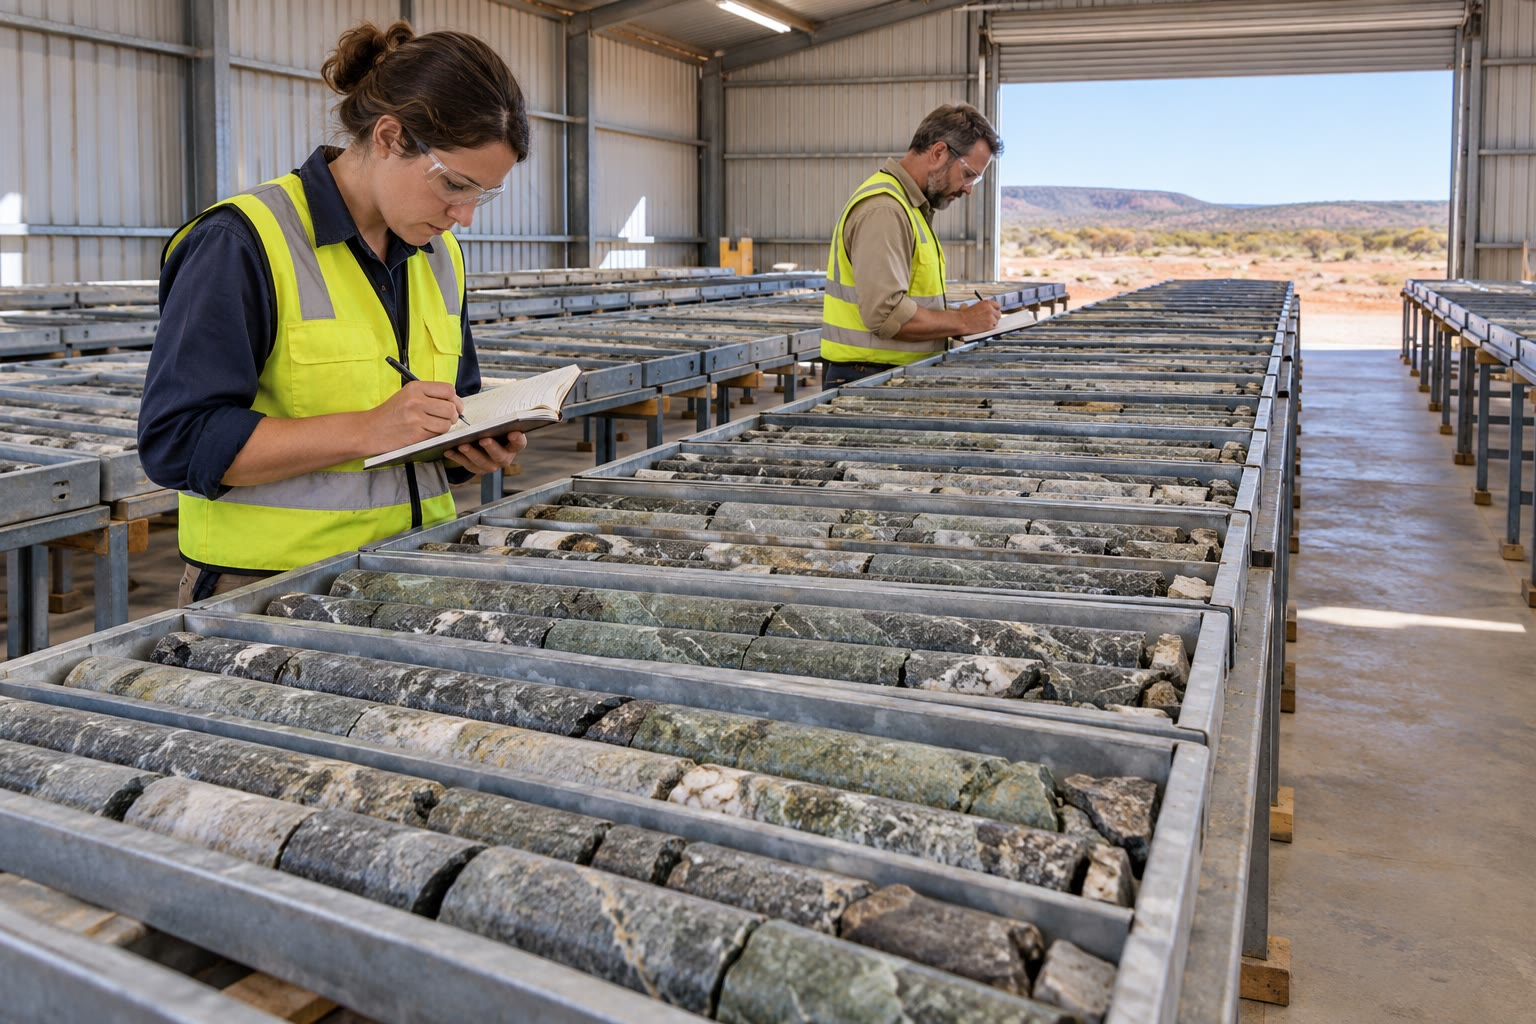
\includegraphics[width=0.56\linewidth]{images/book4/ai/b2-core-shed.jpg}
\par\smallskip{\small किसी अन्वेषण परियोजना में एक कोर-शेड (AI से बनाया गया चित्रण)।}
\par\medskip\raggedright
किसी अन्वेषण परियोजना में हर बोरहोल का कोर धातु की ट्रे में उसी क्रम में बिछाया जाता है जिसमें वह
ज़मीन से निकला। भूवैज्ञानिक ट्रे के साथ-साथ चलते हैं, अंतराल-दर-अंतराल, और दर्ज करते हैं कि चट्टान क्या है,
वह कैसे परिवर्तित हुई है, कौन-सी शिराएँ उसे काटती हैं और किस अनुपात में, और उसमें कौन-से सल्फ़ाइड हैं; वे
चिह्नित करते हैं कि कोर कहाँ आरी से काटा जाएगा और कहाँ से नमूना लिया जाएगा। लॉग आमापनों से पहले आता है
और उनसे मिलाया जाता है: कोई परिवर्तन-क्षेत्र या शिरा-प्रकार जो धातु ले जाता है, वही चीज़ बन जाता है जिसका
एक बोरहोल से दूसरे तक अनुसरण किया जाता है, और लॉग से भूवैज्ञानिक वे खंड-चित्र बनाते हैं जिनसे अगले
बोरहोलों की योजना बनती है।
\end{inthefield}

\section*{अभ्यास}\label{sec:b2:ore-deposits:exercises}

अभ्यासों के आँकड़े, अन्यथा न कहा जाए तो: ऊपरी महाद्वीपीय भूपर्पटी, ताँबा \qty{28}{ppm},
सोना \qty{1.5}{ng/g}, क्रोमियम \qty{92}{ppm}; \cref{sec:b2:ore-deposits:grade-tonnage} की पोर्फ़िरी
ताँबा समष्टि: $\log_{10}$ \omterm{def:b2:ore-deposits:grade}{टनभार} (Mt) का माध्य 2.373 और मानक
विचलन 0.654, $\log_{10}$ ग्रेड (\%) का माध्य $-0.364$ और मानक विचलन 0.199, सहसंबंध
$\rho = 0.100$। तीन सार्थक अंकों तक पूर्णांकित कीजिए।
% ledger: rg03:ucc-trace, data:b4-porphyry-cu

\begin{exercise}[$\star$]\label{exo:b2:ore-deposits:1}
ऊपरी भूपर्पटी के सापेक्ष इनका \omterm{def:b2:ore-deposits:cf}{सांद्रण गुणक} ज्ञात कीजिए: (क)~\qty{0.5}{\percent} वाला एक ताँबा
अयस्क; (ख)~\qty{6}{g/t} वाला एक सोना अयस्क; (ग)~\qty{90}{\percent} क्रोमाइट वाला एक क्रोमाइटाइट,
क्रोमाइट को FeCr$_2$O$_4$ मानकर (परमाणु द्रव्यमान Cr 52.00, Fe 55.85, O 16.00)।
\end{exercise}

\begin{exercise}[$\star$]\label{exo:b2:ore-deposits:2}
बातू हिजाउ को \qty{914}{Mt}, \qty{0.53}{\percent} Cu और \qty{0.40}{g/t} Au पर, बताया गया है, जब कट-ऑफ़
\qty{0.3}{\percent} हो, और उपलब्ध न्यूनतम कट-ऑफ़ पर \qty{1640}{Mt}, \qty{0.44}{\percent} Cu और \qty{0.45}{g/t}
Au पर। (क)~हर अनुमान का अंतर्विष्ट ताँबा (Mt) और सोना (t) ज्ञात कीजिए। (ख)~दूसरे अनुमान के अतिरिक्त खंड
कितना \omterm{def:b2:ore-deposits:grade}{टनभार} और कितना ताँबा जोड़ते हैं, और किस माध्य ग्रेड पर? (ग)~दोनों अनुमान सही
क्यों हैं?
\end{exercise}

\begin{exercise}[$\star$]\label{exo:b2:ore-deposits:3}
स्टोक्स के नियम में व्यास $d$ वाले किसी कण का अवसादन-वेग $(\rho_s -
\rho_w)\,d^2$ के समानुपाती है। $\rho_w = 1.00$, क्वार्ट्ज़ 2.65, सोना 19.3, ज़िरकॉन 4.7 लीजिए (सभी
\unit{g.cm^{-3}} में)। (क)~समान आकार के क्वार्ट्ज़ कण की तुलना में सोने का कण कितने गुना तेज़ी से बैठता है?
(ख)~समान गति से बैठने वाले सोने और क्वार्ट्ज़ के कणों के व्यासों का अनुपात क्या है? (ग)~कौन-सा
क्वार्ट्ज़ कण \qty{0.1}{mm} के ज़िरकॉन कण की तरह बैठता है?
\end{exercise}

\begin{exercise}[$\star$]\label{exo:b2:ore-deposits:4}
एक प्राथमिक ताँबा अयस्क का ग्रेड \qty{0.4}{\percent} है। अपक्षय \qty{150}{m} की मोटाई पर उसका सारा
ताँबा निक्षालित करता है और उसे ठीक नीचे \qty{50}{m} मोटी एक परत में फिर से निक्षेपित करता है, घनत्व
समान रहता है। (क)~परत का ग्रेड ज्ञात कीजिए। (ख)~यही, यदि निक्षालित ताँबे का केवल \qty{80}{\percent}
फिर से निक्षेपित हो। (ग)~पूर्ण पुनर्निक्षेपण के साथ कितनी निक्षालित मोटाई \qty{1.7}{\percent}
देगी?
\end{exercise}

\begin{exercise}[$\star\star$]\label{exo:b2:ore-deposits:5}
किसी \omterm{def:b2:magma-emplacement:magma}{मैग्मा} में \qty{10}{ppb} प्लैटिनम और \qty{200}{ppm} निकेल है; $D_{\mathrm{Pt}} =
10^4$ और $D_{\mathrm{Ni}} = 500$ लीजिए। (क)~\eqref{eq:b2:ore-deposits:r-factor} का उपयोग करके
सल्फ़ाइड में प्लैटिनम (ppm) और निकेल (भार-\%) की मात्राएँ $R = 100$, \num{1000}, \num{10000}
और \num{100000} के लिए ज्ञात कीजिए। (ख)~$R \to \infty$ के लिए उनकी सीमाएँ ज्ञात कीजिए। (ग)~समझाइए कि
निकेल अयस्क $R$ के बारे में कम क्यों बताता है, और प्लैटिनम अयस्क अधिक।
\end{exercise}

\begin{exercise}[$\star\star$]\label{exo:b2:ore-deposits:6}
पोर्फ़िरी ताँबा समष्टि के लिए \eqref{eq:b2:ore-deposits:product} का उपयोग करके: (क)~$\log_{10} M$ का माध्य
और मानक विचलन, और माध्यिका अंतर्विष्ट ताँबा ज्ञात कीजिए। (ख)~निक्षेपों का कौन-सा अंश \qty{10}{Mt} से अधिक
ताँबा रखता है? 422 में से कितने? (ग)~सहसंबंध की उपेक्षा करके (ख) दोहराइए।
\end{exercise}

\begin{exercise}[$\star\star$]\label{exo:b2:ore-deposits:7}
चित्र के दृष्टांत-निक्षेप के लिए ($T_0 = \qty{1000}{Mt}$, माध्यिका \qty{0.40}{\percent},
$s = 0.60$), \eqref{eq:b2:ore-deposits:gt} का उपयोग करके \qty{0.3}{\percent} और \qty{0.6}{\percent} के
कट-ऑफ़ से ऊपर \omterm{def:b2:ore-deposits:grade}{टनभार}, माध्य ग्रेड और अंतर्विष्ट ताँबा ज्ञात कीजिए। चित्र पर एक बिंदु की जाँच कीजिए।
\end{exercise}

\begin{exercise}[$\star\star$]\label{exo:b2:ore-deposits:8}
एक पोर्फ़िरी निक्षेप में \qty{5}{Mt} ताँबा है। मान लीजिए उसका मैग्मीय तरल \qty{1000}{ppm}
ताँबा ले गया, जिसका आधा अयस्क में निक्षेपित हुआ, और \omterm{def:b2:magma-emplacement:magma}{मैग्मा} ने अपने द्रव्यमान का \qty{3.5}{\percent}
तरल के रूप में मुक्त किया। (क)~आवश्यक तरल और \omterm{def:b2:magma-emplacement:magma}{मैग्मा} का द्रव्यमान ज्ञात कीजिए। (ख)~\omterm{def:b2:magma-emplacement:magma}{मैग्मा} का आयतन ज्ञात
कीजिए, जिसका घनत्व \qty{2600}{kg.m^{-3}} है। (ग)~यदि \omterm{def:b2:magma-emplacement:magma}{मैग्मा} में \qty{50}{ppm} ताँबा था, तो उसका कौन-सा
अंश अयस्क में पहुँचा?
\end{exercise}

\begin{exercise}[$\star\star$]\label{exo:b2:ore-deposits:9}
पृष्ठभूमि के आठ सरिता-अवसाद $\log_{10}$ Cu (ppm) के मान 1.30, 1.45, 1.38, 1.52, 1.41, 1.35,
1.48 और 1.40 देते हैं। (क)~लघुगणकों का माध्य और मानक विचलन (समष्टि) ज्ञात कीजिए, और पृष्ठभूमि माध्यिका
तथा देहली (माध्य जमा दो मानक विचलन), ppm में। (ख)~खनिजित भूमि के \qty{4}{km^2} का अपवाह करने वाली
एक सहायक नदी \qty{400}{ppm} वाला अवसाद ले जाती है; वह पृष्ठभूमि माध्यिका वाली, \qty{36}{km^2} का अपवाह
करने वाली एक धारा से मिलती है। यह मानते हुए कि हर वर्ग किलोमीटर अवसाद का समान द्रव्यमान देता है, क्या
मिश्रित अवसाद विसंगत है? (ग)~कुल जलग्रहण क्षेत्र के किस मान तक विसंगति देहली से ऊपर
बनी रहती है?
\end{exercise}

\begin{exercise}[$\star\star\star$]\label{exo:b2:ore-deposits:10}
(क)~$e^{su}\varphi(u) = e^{s^2/2}\varphi(u - s)$ सिद्ध कीजिए। (ख)~किसी लघुगणकीय-प्रसामान्य चर का
माध्य, $e^{\mu + s^2/2}$, निगमित कीजिए। (ग)~दिखाइए कि कट-ऑफ़ से ऊपर धातु का अंश,
$\Phi(z + s)$, \omterm{def:b2:ore-deposits:grade}{टनभार} के अंश $\Phi(z)$ से सदा अधिक होता है, और इसकी व्याख्या कीजिए।
\end{exercise}

\begin{exercise}[$\star\star\star$]\label{exo:b2:ore-deposits:11}
(क)~\eqref{eq:b2:ore-deposits:r-factor} से वह $R$ ज्ञात कीजिए जिस पर $C_S$ अंश $f$ तक पहुँचता है, अपनी
अधिकतम सीमा $D\,C_L$ के सापेक्ष। (ख)~$f = 0.5$ और $0.9$ के लिए इसका मान निकालिए, $D = 300$ (निकेल) और $D =
10^4$ (प्लैटिनम) के साथ। (ग)~पाठ में दिए गए निकेल--ताँबा अयस्कों और प्लैटिनम-समूह तत्त्व
रीफ़ों के $R$ के परासों से तुलना कीजिए।
\end{exercise}

\begin{exercise}[$\star\star\star$]\label{exo:b2:ore-deposits:12}
(क)~किसी लघुगणकीय-प्रसामान्य चर $M$ के लिए, जिसके $\ln M$ का मानक विचलन $s$ है, दिखाइए कि कोटि $q$ के
क्वांटाइल से ऊपर के निक्षेप कुल धातु का $\Phi\bigl(s - \Phi^{-1}(q)\bigr)$ अंश रखते हैं।
(ख)~पोर्फ़िरी समष्टि और $q = 0.9$ के लिए इसका मान निकालिए। (ग)~$q = 0.99$ के लिए भी यही; इसकी तुलना
उन चार सबसे बड़े निक्षेपों से कीजिए जो संकलन के ताँबे का \qty{26.6}{\percent} रखते हैं।
\end{exercise}
% ledger: data:b4-porphyry-cu

\begin{problem}[{सप्ताहांत समस्या --- एक पोर्फ़िरी पूर्वेक्षण-स्थल}]\label{pb:b2:ore-deposits:1}
एक पोर्फ़िरी पूर्वेक्षण-स्थल (काल्पनिक) में बोरहोल खोदे गए हैं। उसके खोज-बोरहोल ने ऊपर से नीचे तक आठ
अंतराल काटे (लंबाई मीटर में, ताँबा ग्रेड प्रतिशत में): 30 m, ग्रेड 0.12; 40, 0.35; 50, 0.62; 60,
0.48; 40, 0.27; 30, 0.81; 50, 0.41; 30, 0.18। सभी बोरहोलों का एक भू-सांख्यिकीय अध्ययन पाता है कि
खंड-ग्रेड लघुगणकीय-प्रसामान्य हैं, माध्यिका \qty{0.38}{\percent} और $s = 0.55$ के साथ, जो $\ln g$ का मानक
विचलन है। खनिजित पिंड \qty{450}{m} त्रिज्या और \qty{700}{m} ऊँचाई के एक ऊर्ध्वाधर बेलन के निकट है, जिसका
घनत्व \qty{2.7}{t.m^{-3}} है। अभ्यासों के आँकड़ों का उपयोग कीजिए, और तीन सार्थक अंकों तक पूर्णांकित कीजिए
(प्रायिकताएँ चार तक)।

\noindent\textbf{भाग I --- खोज-बोरहोल।}
\begin{enumerate}
  \item नमूना लिए गए बोरहोल की लंबाई और उसका लंबाई-भारित माध्य ग्रेड ज्ञात कीजिए।
  \item आठ ग्रेडों का समांतर माध्य ज्ञात कीजिए। भारित माध्य ही सही क्यों है?
  \item लंबाई का कौन-सा अंश \qty{0.3}{\percent} से ऊपर है, और किस माध्य ग्रेड पर?
  \item ऊपरी भूपर्पटी के सापेक्ष भारित माध्य ग्रेड का \omterm{def:b2:ore-deposits:cf}{सांद्रण गुणक} ज्ञात कीजिए।
  \item सबसे समृद्ध अंतराल के लिए भी यही।
  \item निक्षेप के सभी खंडों का माध्य ग्रेड ज्ञात कीजिए। क्या खोज-बोरहोल प्रतिनिधिक है?
\end{enumerate}

\noindent\textbf{भाग II --- कट-ऑफ़ से ऊपर का टनभार।}
\begin{enumerate}[resume]
  \item पिंड का आयतन और \omterm{def:b2:ore-deposits:grade}{टनभार} $T_0$ ज्ञात कीजिए; $T_0 = \qty{1200}{Mt}$ रखिए।
  \item \qty{0.3}{\percent} के कट-ऑफ़ के लिए $z$ और उससे ऊपर के खंडों का अंश ज्ञात कीजिए।
  \item 0.2, 0.3 और \qty{0.5}{\percent} के कट-ऑफ़ से ऊपर का \omterm{def:b2:ore-deposits:grade}{टनभार} ज्ञात कीजिए।
  \item \qty{0.3}{\percent} कट-ऑफ़ से ऊपर का माध्य ग्रेड ज्ञात कीजिए।
  \item 0.2 और \qty{0.5}{\percent} से ऊपर भी यही।
  \item कट-ऑफ़ को 0.3 से \qty{0.5}{\percent} तक बढ़ाने पर \omterm{def:b2:ore-deposits:grade}{टनभार} और माध्य ग्रेड किन गुणकों से
        बदलते हैं?
  \item किस कट-ऑफ़ पर आधा \omterm{def:b2:ore-deposits:grade}{टनभार} रखा जाता है, और उसका माध्य ग्रेड क्या है?
\end{enumerate}

\noindent\textbf{भाग III --- विश्व के पोर्फ़िरी निक्षेपों के बीच यह पूर्वेक्षण-स्थल।}
\begin{enumerate}[resume]
  \item पूरे पिंड में, उसके माध्य ग्रेड पर, अंतर्विष्ट ताँबा ज्ञात कीजिए।
  \item विश्व समष्टि में उसके \omterm{def:b2:ore-deposits:grade}{टनभार} का मानक प्राप्तांक और उसका शतमक ज्ञात कीजिए।
  \item उसके माध्य ग्रेड के लिए भी यही।
  \item सहसंबंध के साथ और उसके बिना $\log_{10} M$ का मानक विचलन ज्ञात कीजिए।
  \item उसके अंतर्विष्ट ताँबे का शतमक ज्ञात कीजिए।
  \item 422 निक्षेपों में से कितनों में इससे अधिक ताँबा होने की अपेक्षा होगी?
\end{enumerate}

\noindent\textbf{भाग IV --- कट-ऑफ़ से ऊपर का ताँबा।}
\begin{enumerate}[resume]
  \item \qty{0.2}{\percent} कट-ऑफ़ से ऊपर अंतर्विष्ट ताँबा ज्ञात कीजिए।
  \item \qty{0.5}{\percent} से ऊपर भी यही।
  \item ताँबे का कौन-सा अंश \qty{0.3}{\percent} से ऊपर है, और \omterm{def:b2:ore-deposits:grade}{टनभार} का कौन-सा
        अंश?
  \item प्रश्न 9 और 20 के उत्तरों का उपयोग करके समझाइए कि कट-ऑफ़ को \qty{0.3}{\percent} से नीचे करने पर
        बहुत चट्टान और थोड़ा ताँबा क्यों जुड़ता है।
  \item सारांश में: पूर्वेक्षण-स्थल में \qty{0.3}{\percent} कट-ऑफ़ से ऊपर कितना ताँबा है?
\end{enumerate}
\end{problem}
